% ***********************************************************
% ******************* PHYSICS HEADER ************************
% ***********************************************************
% Version 2
\documentclass[11pt]{article} 
\usepackage{amsmath} % AMS Math Package
\usepackage[utf8]{inputenc}
\usepackage[T1]{fontenc}
\usepackage{subfiles}
\usepackage{hyperref}
\usepackage{amsthm} % Theorem Formatting
\usepackage{amssymb}	% Math symbols such as \mathbb
\usepackage{graphicx} % Allows for eps images
\usepackage{multicol} % Allows for multiple columns
\usepackage[dvips,letterpaper,margin=0.75in,bottom=0.5in]{geometry}
 % Sets margins and page size
\pagestyle{empty} % Removes page numbers
\makeatletter % Need for anything that contains an @ command 
\renewcommand{\maketitle} % Redefine maketitle to conserve space
{ \begingroup \vskip 10pt \begin{center} \large {\bf \@title}
	\vskip 10pt \large \@author \hskip 20pt \@date \end{center}
  \vskip 10pt \endgroup \setcounter{footnote}{0} }
\makeatother % End of region containing @ commands
\renewcommand{\labelenumi}{(\alph{enumi})} % Use letters for enumerate
% \DeclareMathOperator{\Sample}{Sample}
\let\vaccent=\v % rename builtin command \v{} to \vaccent{}
\renewcommand{\v}[1]{\ensuremath{\mathbf{#1}}} % for vectors
\newcommand{\gv}[1]{\ensuremath{\mbox{\boldmath$ #1 $}}} 
% for vectors of Greek letters
\newcommand{\uv}[1]{\ensuremath{\mathbf{\hat{#1}}}} % for unit vector
\newcommand{\abs}[1]{\left| #1 \right|} % for absolute value
\newcommand{\avg}[1]{\left< #1 \right>} % for average
\let\underdot=\d % rename builtin command \d{} to \underdot{}
\renewcommand{\d}[2]{\frac{d #1}{d #2}} % for derivatives
\newcommand{\dd}[2]{\frac{d^2 #1}{d #2^2}} % for double derivatives
\newcommand{\pd}[2]{\frac{\partial #1}{\partial #2}} 
% for partial derivatives
\newcommand{\pdd}[2]{\frac{\partial^2 #1}{\partial #2^2}} 
% for double partial derivatives
\newcommand{\pdc}[3]{\left( \frac{\partial #1}{\partial #2}
 \right)_{#3}} % for thermodynamic partial derivatives
\newcommand{\ket}[1]{\left| #1 \right>} % for Dirac bras
\newcommand{\bra}[1]{\left< #1 \right|} % for Dirac kets
\newcommand{\braket}[2]{\left< #1 \vphantom{#2} \right|
 \left. #2 \vphantom{#1} \right>} % for Dirac brackets
\newcommand{\matrixel}[3]{\left< #1 \vphantom{#2#3} \right|
 #2 \left| #3 \vphantom{#1#2} \right>} % for Dirac matrix elements
\newcommand{\grad}[1]{\gv{\nabla} #1} % for gradient
\let\divsymb=\div % rename builtin command \div to \divsymb
\renewcommand{\div}[1]{\gv{\nabla} \cdot \v{#1}} % for divergence
\newcommand{\curl}[1]{\gv{\nabla} \times \v{#1}} % for curl

\newcommand{\laplace}[1]{\Delta #1} % for laplacian
\newcommand{\eps}{\epsilon_0} % electric permittivity
\newcommand{\oneover}[1]{\frac{1}{#1}} % 1/thing
\newcommand{\dotproduct}[2]{\v{#1} \cdot \v{#2}} % for dotproduct
\newcommand{\crossproduct}[2]{\v{#1} \times \v{#2}} % for crossproduct
\newcommand{\fourierv}[1]{\tilde{\v{#1}}}
%aliases
\newcommand{\para}{\parallel}
\newcommand{\rot}[1]{\curl{#1}}

\let\baraccent=\= % rename builtin command \= to \baraccent
\renewcommand{\=}[1]{\stackrel{#1}{=}} % for putting numbers above =
\newtheorem{prop}{Proposition}
\newtheorem{thm}{Theorem}[section]
\newtheorem{lem}[thm]{Lemma}
\theoremstyle{definition}
\newtheorem{dfn}{Definition}
\theoremstyle{remark}
\newtheorem*{rmk}{Remark}

% ***********************************************************
% ********************** END HEADER *************************
% ***********************************************************
\usepackage[utf8]{inputenc}
\usepackage{graphicx}
\title{Notes from PlasmaX}
\author{Perfi}

\begin{document}
\maketitle

These notes will not be $100\%$ comprehensive, as I'm making them mainly for my own use. However, if you spot any mistakes, feel free to catch me on the forums and I'll fix any mistakes. 

\section{Week 1. Description of the plasma state, with Paolo Ricci}
Didn't start making notes until 1.5 so I'll be skimming the earlier topics.
	\subsection{Plasmas in nature and laboratory}
		\begin{itemize}
			\item Plasma - the 4th state of matter. Heat stuff up to ~11400K (= 1eV) and gases begin being ionized.
			\item The Sun is a miasma of incandescent plasma\footnote{\text{https://www.youtube.com/watch?v=sLkGSV9WDMA}}
			\item Lightning is plasma (ionized air)
			\item Plasma diplays
			\item Nuclear fusion - can't really get there without turning stuff into plasma
	\item The word `plasma' comes from greek $\pi\lambda\alpha\sigma\mu\alpha$, which means `moldable substance' or `jelly', though it was mentioned on the forums that it might mean `living thing'... which is really fitting when you think about it
			\item A brief history:
				\begin{itemize}
					\item 1920's-1930's: ionospheric plasma research (for radio transmission) and vacuum tubes (Langmuir)
					\item 1940's: MHD plasma waves (Alfvén)
					\item 1950's: research on Magnetic Fusion. Geneva UN conference on uses for atomic energy which don't kill people
				\end{itemize}
			\item Fusion experiments: L-1, TFTR, JET, ITER tokamaks; W7-X stellarator at MPI in Germany; the NIF inertial fusion facility in US
			\item The Earth's magnetosphere; van Allen belts
			\item Jets - space plasmas
			\item Lots of industrial applications
		\end{itemize}
		
	\subsection{Rigorous definition of plasma: Debye length}
	A plasma is a \textbf{globally neutral} \emph{ionised gas} with \textbf{collective effects}

	The following parameters classify plasmas:
		\begin{itemize}
			\item \textbf{Debye length}
			
			Distance over the potential of a charged particle decreases by a factor $1/e$ due to screening by other charged particles
			
			\[\lambda_{De} = \sqrt{\frac{\epsilon_0 T_e}{e^2 n_0}} \] (for electrons)
			
			Solved in lecture by a statistical approach which assumed $n\frac{4}{3}\pi \lambda_{De}^3 \equiv N_D \gg 1$ (for a Debye sphere; in the lecture $n \lambda_{De}^3$ was used, which relates to a Debye cube. There's not much difference between them, a factor of $~4$). $N_D$  means the number of particles inside a sphere (or cube, following the lecture) of radius equal to the Debye length. The condition means there's plenty of particles to screen our test particle. This also assumed that binary interactions between particles were weak ($\frac{e \phi}{T_e} \gg 1$)
			\end{itemize}
	\subsection{Plasma definition: frequencies and parameters}
\begin{itemize}
\item \textbf{Plasma frequency}
Assume a plasma of same density of ions and electrons. Displace electrons by $\Delta x$. They begin to exhibit harmonic oscillations (for $\Delta x$ not too large). Newton's 2nd law gives
\[\dd{\Delta x}{t} + \frac{n_0 e^2}{\epsilon_0 m_e}\Delta x = 0\]
Can define plasma frequency
\[\omega_{pe}\equiv\sqrt{\frac{n_0 e^2}{\epsilon_0 m_e}}=\frac{v_{th,e}}{\lambda_{De}}\]
where $v_{th,e}$ denotes the thermal speed of electrons
\item \textbf{Collision frequency}
	
	The frequency of coulomb collisions between particles
	\[\nu_{coll} \equiv \frac{n_0 e^4}{16 \pi \epsilon_0^2 m_e^2 v_{th,e}^3}\]
	
	\item Size of plasma has to be much larger than its Debye length (or there's no quasineutrality)
	\end{itemize}
	
	\subsection{Particle motion in a static uniform magnetic field . Plasma magnetic properties} 
		\begin{itemize}
			\item Larmor radius - particles gyrate around the guiding center at this distance
			\[\rho \equiv \frac{m v_{\perp}}{\abs{q} B}\]
			\item Cyclotron frequency
			\[\omega_c \equiv \frac{v_{\perp}}{\rho} = \frac{\abs{q} B}{m}\]
			
			Particle rotation direction on their helical trajectory
			\begin{itemize}
			\item $q>0$ (`by default'): left hand rotation with respect to $\v{B}$
			\item $q<0$ (electrons): right hand rotation
			
			\item Magnetic moment
			\[\abs{\v{\mu}} \equiv I A = \frac{\abs{q}\omega_e}{2\pi} \pi \rho^2 = \frac{m v_{\perp}^2}{2 B} = \frac{E_{kin \perp}}{B}\]
			
			(direction opposite to B)
			is an adiabatic invariant for every particle; doesn't change under slow changes of factors. However, it will change through heat exchange, which usually operates on slower timescales than magnetic field changes.
			
			Plasmas are diamagnetic (they reduce externally applied magnetic fields) (because of direction of $\mu$)
			\end{itemize}
		\end{itemize}

	\subsection{Particle motion in given electromagnetic fields: the drifts }
Static and uniform E and B fields. Particles under Lorentz force which can be decomposed as:
	\begin{itemize}
		\item Parallel direction: \[m\d{\v{v_{\parallel}}}{t}=qE_{\parallel}\]
	Uniform acceleration
		\item Perpendicular direction: \[m\d{\v{v_{\perp}}}{t}=q(\v{E_{\perp}} + \v{V_{	\perp}}\times\v{B})\]
	\end{itemize}
The many drifts in a plasma:
	\begin{itemize}
		\item $\v{E}\times\v{B}$ drift
		\begin{itemize}
			\item Perpendicular component averages out over gyroperiod
			\[\v{v_e}=\frac{\v{E_{\perp}}\times\v{B}}{B^2}\]
			\item This is a motion of the guiding center which is superposed over the gyromotion
			\item Does not depend on charge, neither in magnitude nor in direction (but gyromotion direction does)
			\item Guiding center moves over lines of constant electrostatic potential $\phi$ (the drift does not change the particle energy!)
			\item A generalization of this drift for any force: \[\v{v_F}=\frac{\v{F_{\perp}}\times\v{B}}{qB^2}\]
			\item For a gravitational force (say, space plasmas), this depends on charge. Separates positive and negative charges. Polarizes the plasma, creating a $\v{E}$ field and an $\v{E}\times\v{B}$ drift
		\end{itemize}
		
		\item Curvature drift
		\begin{itemize}
			\item \v{B} field curved, particle follows the B field - this happens through a centrifugal force
			\[\v{F_c}=\frac{m v_{\parallel}^2}{R_B^2} \v{R_B}\]
			\item This causes a drift:
			\[\v{v_d} = \frac{\v{F_c} \times \v{B}}{q B^2} = \frac{m v_{\perp}^2}{q B^2 R_B^2} (\v{R_B} \times \v{B})\]
		\end{itemize}
		
		\item Gradient drift $\grad{B} \perp \vec{B})$
		\begin{itemize}
		\item	Happens in changing (spatially) magnetic fields
		\[\v{v_{\grad{B}}} = \frac{m v^2}{q c B^2} (\v{B} \times {\grad{B}} ) \]
			\item A derivation so complicated, it deserved a separate appendix.
			As particles gyrate, they move between regions of smaller and bigger B.
			This causes a drift in a direction perpendicular to both the B field and the gradient of its value
			We consider a small variation in B and expand B in a taylor series around $B_0$.
			
			Then we use that expansion to solve $m \d{\v{v}}{t} = q {\v{v} \times {B}}$, plugging in our expansion for B.
			
			We also decompose the velocity: an average $v_{0}$ and a small perturbation. $v_{0}$ is the solution to the equation for constant magnetic field $B_{0}$.
			
			We neglect the cross product of the two small perturbations and average over a gyroperiod.
			
			We use our knowledge of the solution for the static magnetic field (gyration in the plane perpendicular to B) to deal with the perpendicular velocities (x and y in this decomposition under the assumption that B is along z).
			
			The drift velocity is the perturbation described by the formula above for an arbitrary geometry of the problem.
		\end{itemize}
	\end{itemize}
	
	
	\subsection{Plasma confinement based on single particle motion. Magnetic mirrors, stellarators, tokamaks}
	\begin{itemize}
	\item How do you confine a plasma?
	
	\textbf{Charged} particles follow helical trajectories along B field. This confines them in the perpendicular direction. What about the parallel one?
	\item Can use open field lines. Take two circular coaxial electromagnets.
	
	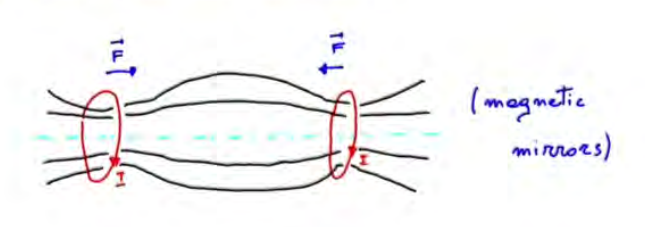
\includegraphics[width=\linewidth]{magneticmirror}
	
	\item Can use closed field lines. Closed geometries. Example: tokamaks (toroidal), stellarators.
	
	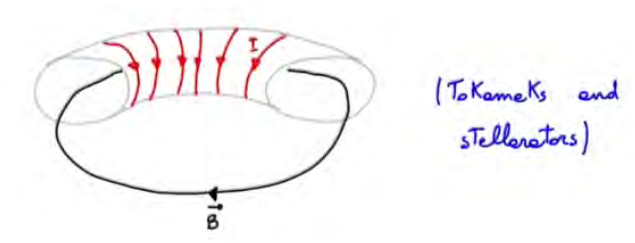
\includegraphics[width=\linewidth]{tokamakconfinement}
	
	\item The magnetic mirror geometry is neat for particles really close to the axis. B is maximum (field density increases) near the electromagnets
	
	force in the axial direction is \[F_z =-\mu\abs{\grad{B}}\]
	
	$v_{\parallel}$ has to vanish at $B_{max}$ so that the kinetic energy is just composed of the perpendicular component of velocity
	
	Particle reflection condition
	\[\frac{v_{\perp}^2}{v_{\perp}^2+v_{\parallel}^2} > \frac {B_{min}}{B_{max}}\]

	
	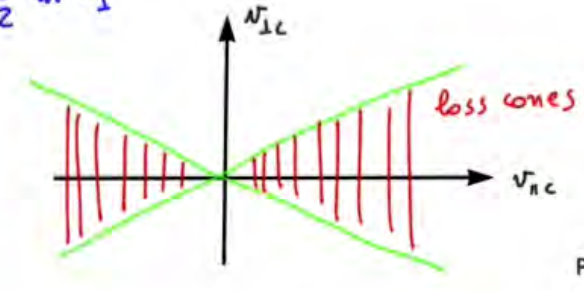
\includegraphics[width=\linewidth]{1f4}
	
	This means that particles in the \textbf{loss cones} in phase space (marked red; those which don't satisfy the inequality) cannot be confined in the mirror!
	
	Neat example: the Earth's magnetic field is a magnetic mirror!
	
	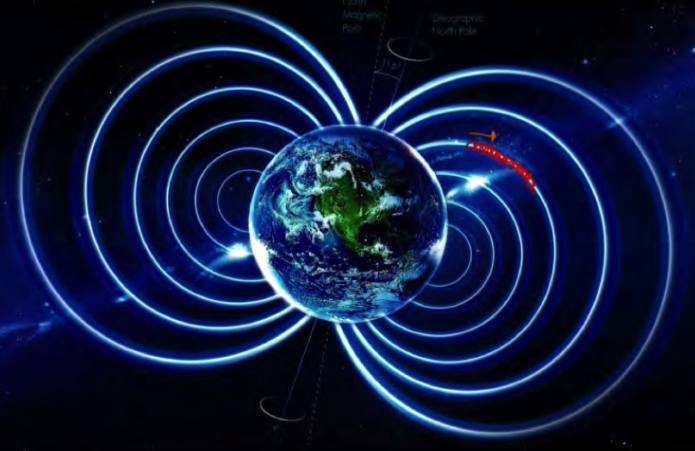
\includegraphics[width=\linewidth]{1f5}

\item What about closed magnetic field lines? Can those deal with loss cones?

B is not homogeneous! Curved! Has curvature and gradient drifts!

For a purely toroidal field, positively charged particles drift towards the bottom, while negatively charged ones drift towards the top. This polarizes the plasma and introduces the $E \times B$ drift outwards, sending the plasma crashing into the major radius wall.

A solution: a poloidal magnetic field to short circuit the charge accumulation. Either:
\begin{itemize}
\item Drive a current through the plasma $\rightarrow$ Tokamaks
\item Get rid of axial symmetry $\rightarrow$ Stellarators
\end{itemize} 

	
	\end{itemize}

%%WEEK 2%%
\section{Week 2: Kinetic description of plasmas, with Paolo Ricci}
\subsection{2a) From single particle to kinetic description }
	Kinetic description of plasma. A (relatively?) complete description of plasma which covers both the particles and the fields evolving over time.

The usual diagram for a plasma description, seen often in simulations:
\begin{enumerate}
	\item Take Newton's equations using electric and magnetic fields \textbf{for all particles at all times} (use Lorentz force)
	\item Use positions and velocities to compute charge and current densities. Charge density given as sum over particles of their charges, localized through use of Dirac delta functions. Current density - similar, but multiplied by particle velocity vectors inside the sum.
	\item Take charge and current density, plug them into Maxwell equations, calculate E and B fields at positions
	\item Take calculated E and B fields and apply them as forces to particles. Repeat cycle until bored or simulation returns segmentation fault.
\end{enumerate}
But real plasmas involve on the order of $10^21$ particles for a fusion plasma. Too much strain on our computational abilities. Impractical. We use a distribution function:

$f(\v{r}, \v{v}, t) d\v{r} d\v{v} = $ number of particles at time t, in phase space volume $d\v{r} d\v{v}$ located at $\v{r}, \v{v}$. We have a separate distribution function $f_i$ for every species
\begin{itemize}
\item Total number of particles $N_S$ given by integral of distribution function over all positions and velocities (which covers all the phase space)
\item Number density of particles $n_s$ given by integral over all velocities for a given location $\v{r}$ 
\item Average velocity given by $\frac{1}{n_s} \int \v{v} f_i(\v{r}, \v{v}, t)  d\v{v}$
\end{itemize}
\par \textbf{Examples of distribution functions}
\begin{itemize}
	\item Maxwell-Boltzmann distribution function, for three dimensions
	\[ F_0(\v{v}) = n_0 (\frac{1}{2 \pi v_{thermal}})^(3/2) exp(-\frac{v^2}{2 v_{thermal}^2}) \] %insert equation
	In 1D, only the normalization of the distribution changes from the 3D case:
	\[ F_0(v) = n_0 (\frac{1}{2 \pi v_{thermal}})^(1/2) exp(-\frac{v^2}{2 v_{thermal}^2}) \]
	\item Monoenergetic beam in 1D
	\[ F_0(v) = n_0 \delta (v-v_0) \]
	\item Two counterstreaming beams in 1D (two-stream instability!)
	\[ F_0(v) = \frac{n_0}{2} [\delta (v-v_0) + \delta(v+v_0)] \]
\end{itemize}

\textbf{Conservation of particles number}

If there are no sources or sinks, we have the following condition for conservation of number of particles
\[ \d{f_s}{t} = -\nabla_{ED} \cdot (\v{u} f_s) \]
where
\[ \nabla_{ED} = ( \d{}{x},\d{}{y},\d{}{z},\d{}{v_x},\d{}{v_y},\d{}{v_z}) = (\d{}{\v{r}}, \d{}{\v{v}}) \]
\[ \v{u} = (\d{\v{r}}{t}, \d{\v{v}}{t}) = (\v{v}, \frac{\v{F}}{m_s}) = (\v{v}, \frac{\v{F_{long range}} + \v{F_{short range}}}{m_s}) \] %insert

Long range forces - collective interactions. Short range forces - binary collisions (between individual particles, like you'd have in a gas).
Plugging these back into the particle conservation equation:
\[ \d{f_s}{t} = -\d{}{\v{r}} \cdot (\v{v} f_s) - \d{}{\v{v}} \cdot [\frac{\v{F_{long range}} + \v{F_{short range}}}{m_s} f_s] \]

\textbf{Boltzmann equation}
	We can improve on the previous equation. Start out with the expanded particle conservation equation:
	
\[ \d{f_s}{t} = -\d{}{\v{r}} \cdot (\v{v} f_s) - \d{}{\v{v}} \cdot [\frac{\v{F_{long range}} + \v{F_{short range}}}{m_s} f_s] \]

\begin{itemize}
	\item In the phase space approach, velocity is treated as a completely independent variable than v (though you could consider one as a derivative of the other). Thus $\d{}{\v{r}} \cdot (\v{v} f_s) = \v{v} \cdot	\d{f_s}{\v{r}}$
		\item long range force can be decomposed into electric field independent of v, and the  $\v{v} \times \v{B}$ term - perpendicular to v. Thus, $\d{}{\v{v}} \cdot [\v{F_{long range}} f_s] = \v{F_{long range}}\cdot\d{f_s}{\v{v}} $
	\item Plugging in:
	
	\[ \d{f_s}{t} = -\v{v}\cdot\d{f_s}{\v{r}} - \frac{\v{F_{long range}}}{m_s} \cdot \d{f_s}{\v{v}} - \d{}{\v{v}} \cdot (\frac{\v{F_{short range}}}{m_s} f_s) \]
	\item Can be rewritten as:
	
	\[ \d{f_s}{t} +\v{v}\cdot\d{f_s}{\v{r}} + \frac{\v{F_{long range}}}{m_s} \cdot \d{f_s}{\v{v}} = - \d{}{\v{v}} \cdot (\frac{\v{F_{short range}}}{m_s} f_s) \]
	
	Term on the right is called a `collision operator' $(\d{f}{t})_c$.	
	
\item And we get the \textbf{Boltzmann equation}:
	\[ \d{f_s}{t} +\v{v}\cdot\d{f_s}{\v{r}} + \frac{q_s}{m_s}(\v{E_{long range}} + \v{v} \times \v{B_{long range}}) \cdot \d{f_s}{\v{v}} = (\d{f_s}{t})_c \]
\end {itemize}

\[   \]

\end{document}
